%!TEX root = vivek-talk.tex 

% General Goal: I want to promote my work. 
% General Goal: Tell audience that what I'm doing is relevant. 
% Specific Goal: Tell audience that low-overhead scheduling can
% benefit the energy efficiency for the product/application that you
% are creating - making money for the company.


\comments{
\begin{frame}
\frametitle{CSE Applications On Supercomputers} 
\begin{itemize}

\item \small Focus of talk is computational science and engineering (CSE) applications
\end{itemize} 
\end{frame}
}

% \begin{frame}{Dissertation Work}

\begin{frame}
\frametitle{Work for Dissertation} 
%\todo{Change to a rough outline such that it doesn't give away storyline.}

\begin{enumerate}
\item Introduction
\item Motivation for Schedulers
\item Lightweight Scheduling with further optimizations + Scalability  
\item Scheduling for Both Transient and Persistent Load imbalances
\item Model-guided Optimization and Optimizations taking into account MPI Slack
\item Balancing Load Balance and Locality in different dimensions
\item Combining all schedulers: Application Programmer Usage
\item Conclusions and Future Work
\end{enumerate} 
\end{frame} 

\begin{frame}[label=modelMPICode]
  \frametitle{Model MPI Code} 
 Common pattern in CSE application codes.\\
%including
  \vspace*{0.1in}
\lstinputlisting{listings/1DstencilUsingMPI.c}
 
\begin{itemize}
%\small \item \small Simulations, characterized by timesteps and/or
%iterations.
\small \item \small Modern machines have multi-core nodes.
\begin{itemize}
\item \small Use a separate MPI process on each core, or 
\item \small Use one or two MPI processes on each node and used shared
  memory parallelism within each process.
\end{itemize}
\item \small Even when the work assigned to each process is identical, there can still be a performance problem.
\end{itemize} 
\end{frame}

%TODO: justify why these old graphs are fine  
\begin{frame}   
\frametitle{Histogram Showing Performance Variation of Reg. Mesh Computation}
\begin{figure}
\begin{center}                     
%(- Add latest histograms here -)    
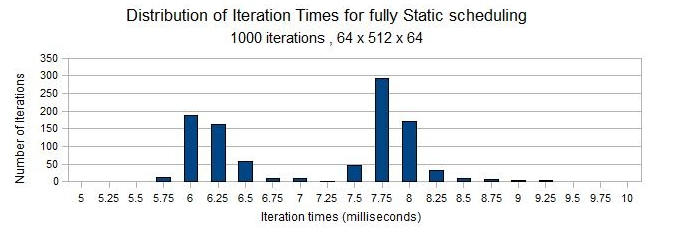
\includegraphics[scale=0.24]{plots/IterTimingsHisto-static}\\ 
%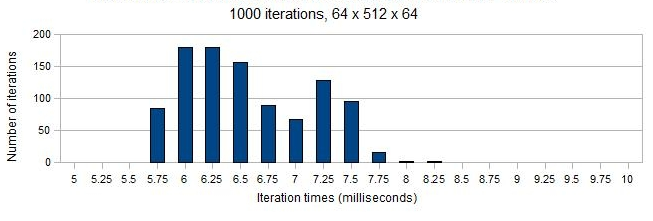
\includegraphics[scale=0.24]{../images/IterTimingsHisto-dynamic}  
\end{center}    
{\small Iteration timings distribution across 1000 timesteps for a reg. mesh computation, for static scheduling \comments{(top) and dynamic scheduling (bottom).}} 
\end{figure} 
\begin{center} 
{\small $\rightarrow$ \textcolor{gray}{Bi-modal distribution for static scheduling.} \comments{Uni-modal distribution for dynamic scheduling, but increased spread and higher mean for dynamic scheduling.} } 
\end{center} 
\end{frame}                                     

\begin{frame}[label=transImbMitigation]
\frametitle{Transient Load Imbalance and its Mitigation} 
\textit{Application timeline schematics.} 
\begin{columns}
\column{0.5\columnwidth}
%\visible<1->{
{\small Infrequent noise $\rightarrow$ slowdown at scale.}
%}
%TODO: slowdown? 
\column{0.5\columnwidth}
%\visible<1->{
{\small \comments{$\exists$ large \# cores / node $\rightarrobw$} Idea for fix: redistribute within node.}
%}
\end{columns}

%TODO: animate this to show right one slide later.
%\visible<1->{
\begin{figure}[ht!]
  \label{fig:NoiseTransImbPic}
\subfloat[\label{fig:AmplificationPic1} \small Noise delays almost every iteration.]{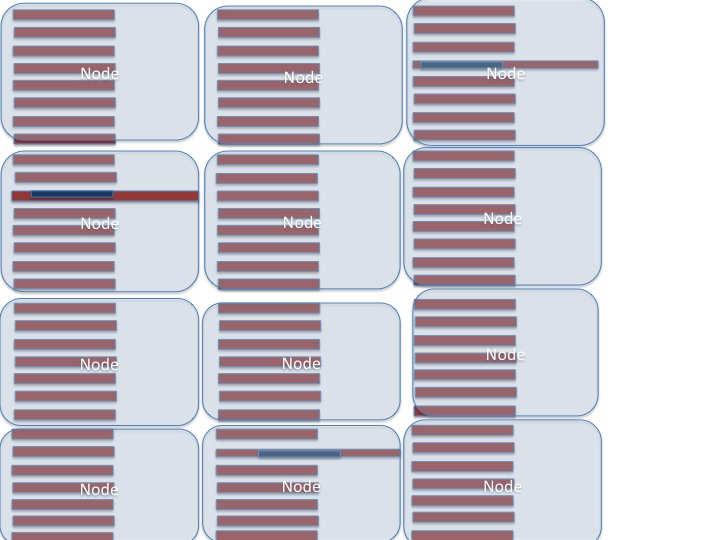
\includegraphics[height=1.3in]{pictures/Noise}}
%  }
  
%\visible<1->{
\hspace*{0.25in}\subfloat[\label{fig:AmplificationPic3}{\small Performance improves, assuming perfect work re-distribution within each node.} %can be perfectly re-distributed within each node. 
]{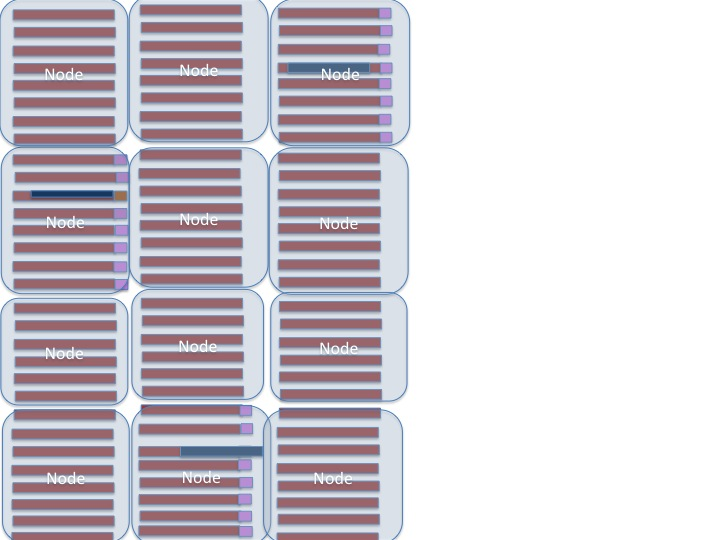
\includegraphics[height=1.3in]{pictures/NoiseMitigated}}
%}
\caption{\label{fig:NoiseTransImbPic} Application timeline schematics.}
\end{figure}
%\todo{S: This should not be a Figure.. 'Figure 1'looks out of place in a presentation} 
\end{frame}

\begin{frame} 
\frametitle{Amplification Problem in the Context of System Noise}          
\begin{itemize}  
\item \small On one node running 1000 timesteps of length 10 ms.            
\begin{itemize}  
\item \tiny Assume: Perf. irregularity (PI) is of length 5 ms, and it occurs approximately every second.
\item \tiny Execution time without PI 10 ms * 1000 timesteps = 10 seconds. 
\item \tiny With PI: 10 out of 1000 timesteps will be affected (that is delayed by 5 ms) .  So, the total delay is 50 ms. 
\item \tiny Execution time is 10.05 seconds, i.e., 0.5\% delay.  
\end{itemize} 
\item \small  On two nodes (weak scaling):   
\begin{itemize}    
\item \tiny Probability that an iteration is delayed on one of the nodes is 1\%, same as above.  
\item \tiny Probability that a given iteration is delayed on any processor is : $1.0 - (1 - 0.01)^2$  =  $1.99$\% .
\item \tiny The delay is then $1000 \times 0.0199 \times 5$  = $99.5$ ms for a total execution time of $10.0995$ s.
\end{itemize}             
\item \small On p nodes :    
\begin{itemize}   
\item \tiny The delay is $1000 \times (1.0 - 0.99^p) \times 5$ ms       
\item \tiny For 10 nodes:$1000 \times 0.0956 \times 5$ ms =  478 ms                                     
\item \tiny For 100 nodes: $1000 \times 0.634 \times 5$ ms = 3170 ms               
\item \tiny For 1000 nodes:  $1000 \times 0.9999 \times 5$ = 4999.5 ms                                  
\end{itemize}                         
\item \small That's a 50\% performance loss.   
\item \small As p increases, the probability that one node experiences a delay on a given iteration starts approaching 100\%. 
\end{itemize}  
\end{frame}    


\begin{frame}[label=mitigationWithinNode]
\frametitle{Within-node Persistent Load Imbalance and Mitigation}
\begin{figure}[ht!]
\label{fig:AppPersistentImbPic}
\subfloat[\tiny Application imbalances.]{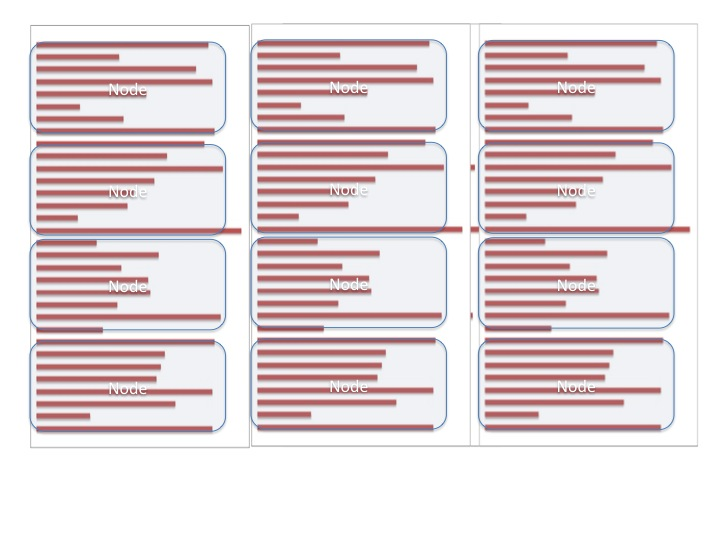
\includegraphics[height=1.3in]{./pictures/PersistentImb2}}\label{fig:AmplificationPic3}\hspace*{0.25in}\subfloat[\label{fig:AmplificationPic3}\tiny Mitigated by within-node re-distribution.]{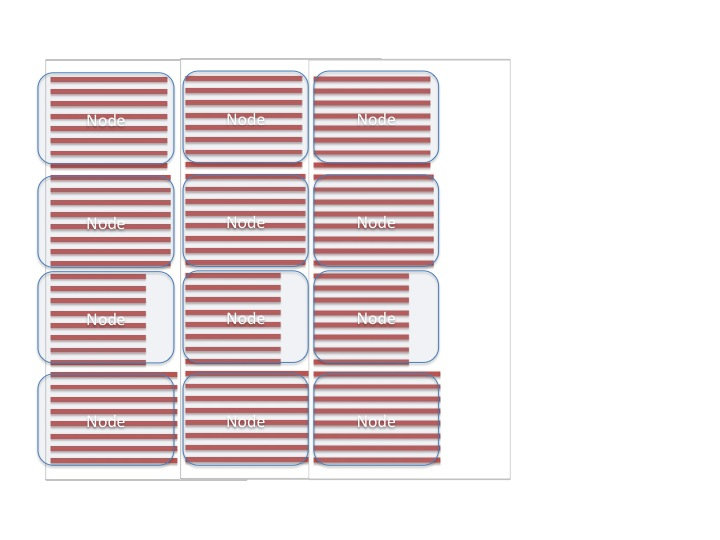
\includegraphics[height=1.3in]{./pictures/PersistentOptimized}}
%\caption{\label{fig:AppPersistentImbPic} Application-induced load imbalances.}
\end{figure}
{\small Indent due to not doing across-node balancing but still much better than before.}
\end{frame}

%TODO: see if we can change title
\begin{frame}[label=dynLoadBal]
\frametitle{So, can dynamic load balancing fix this?}
\begin{itemize}
\item \small Dynamic load balancing within a node has potential to mitigate imbalances, {\it if} it can be done efficiently.
%\item Dynamic
%\begin{itemize}
%\item For both kinds of imbalances.
%\item \small Persistent imbalance can also be addressed by across-node
%  balancing (avail. in Charm++, Zoltan), but it requires more complex
%  machinery (and is complementary anyway).\\
%know questions here
%\end{itemize}
\item \small OpenMP supports dynamic balancing.
\item \small Let us use OpenMP within-node.
\vspace*{.5in}
%\item However, within-node dynamic load balancing faces many challenges. 
\end{itemize}
\end{frame}

% Good because it's concrete . 
%TODO: add in the mpi. 
%TODO: fix labels. 
%TODO: word the expected overhead of idle time better.
%TODO: check cause/challenge here and in thesis. 
\begin{frame}[label=execTimings]
\frametitle{Execution Timings Breakdown}
{\tiny \textbf{\underline{Setup:}} One process per node, binding, gcc
with -O3, gomp runtime, one Intel Xeon 16-core node of LLNL cluster
named cab, each data point in the graph found from average of five independent timings.}\\

% TODO:L0: figure out whether we should add data on 4 MPI processes per
% node, i.e., 1 MPI process per socket. 
% TODO: L0: check whether to include thread to core binding 
% TODO: L0: check the five timings. Is it 3 ? Should it be 20 ? 
% TODO: L3: explain that you ran the application code this way -
% important to tell to explain our findings . and assumptions.. 
% TODO: L4: fix wording of 'ran on one Intel Xeon 16-core node - take
% from previous slides. 

\begin{figure}[ht!]
\label{fig:dmTimes-cab}
\begin{center}
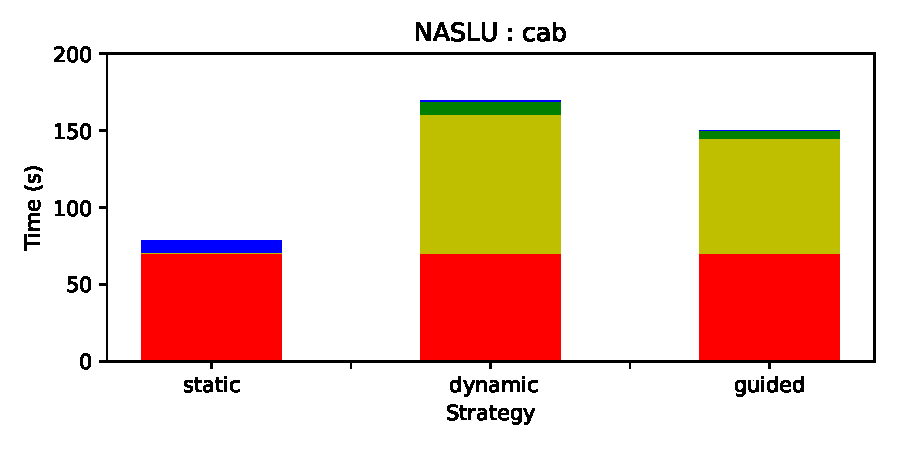
\includegraphics[scale=0.35]{./plots/dmTime-NASLU-cab}
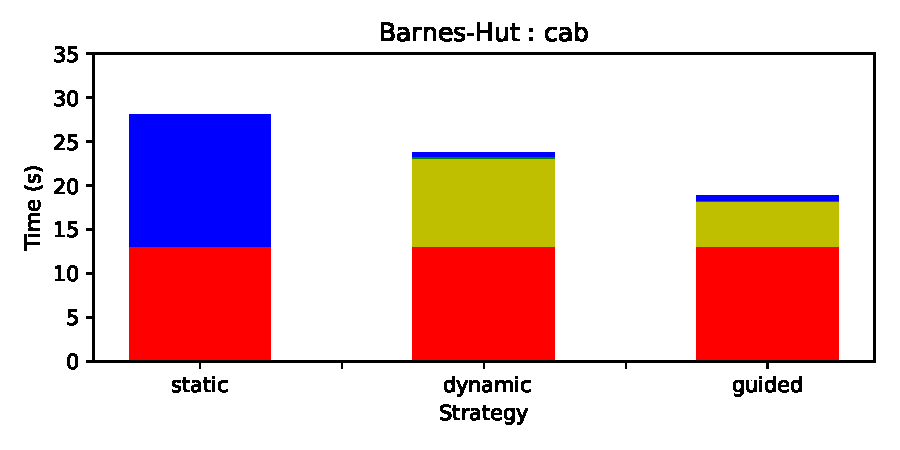
\includegraphics[scale=0.35]{./plots/dmTime-nbody-cab}
\end{center}
\caption{\label{fig:dmTimes-cab} \tiny Breakdown of time. Computation in red, idle in blue, synchronization in green.}
\end{figure}
\begin{enumerate}
\small \item \small Idle time eliminated with dynamic
\small \item \small Synchronization overheads for dynamic: small,
although significant ($\approx$ 5\%).
\item \small Most of the overhead (shown in yellow) must be data movement.
%\item \tiny While seemingly insignificant, they account for roughly 5\% percent of execution time for both of these applications. 
\end{enumerate}
\end{frame}

\begin{frame}[label=dataMovement]
\frametitle{Data Movement}
{\tiny Measured L2 and L3 cache misses with PAPI.}
\visible<1->{
\begin{figure}[t]
\label{fig:cacheMisses-cab} 
\begin{center}
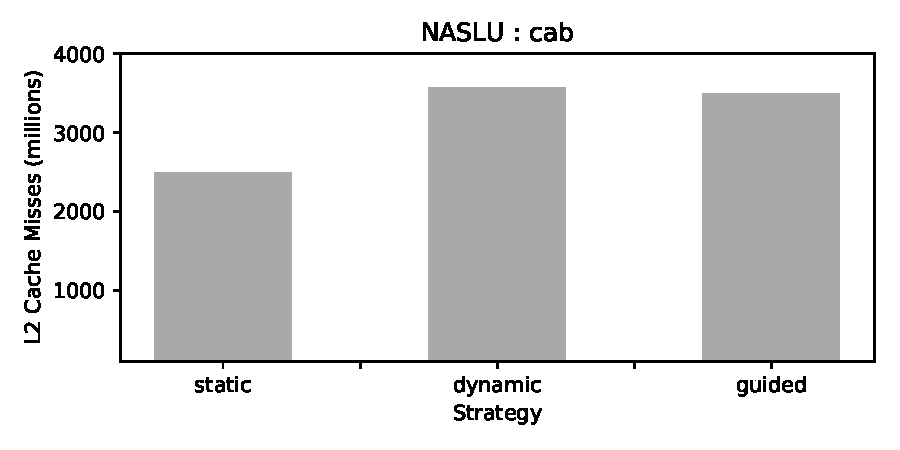
\includegraphics[scale=0.30]{./plots/L2-cacheMisses-NASLU-cab}
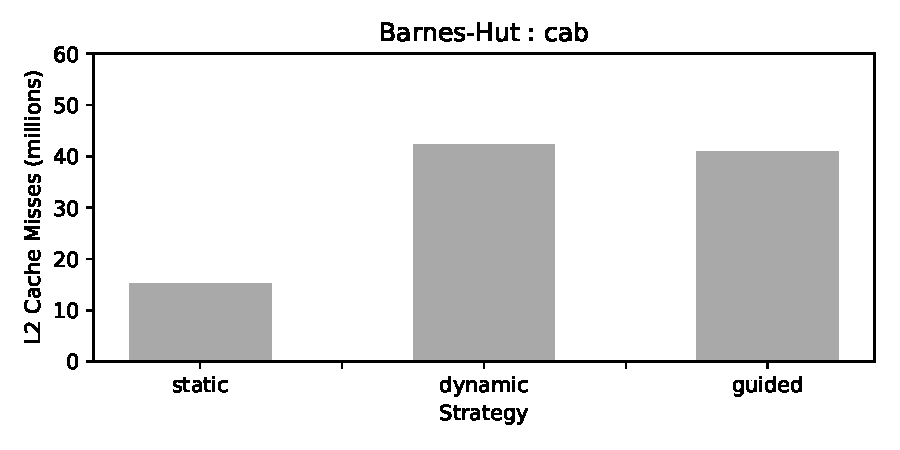
\includegraphics[scale=0.30]{./plots/L2-cacheMisses-nbody-cab}\\
%\includegraphics[scale=0.30]{./plots/L3-cacheMisses-NASLU-cab}
%\includegraphics[scale=0.30]{./plots/L3-cacheMisses-nbody-cab}
\end{center}
\end{figure}
\begin{center}
{\tiny Cache misses with L2 misses on top for different OpenMP scheduling strategies.}
\end{center}}
\visible<1->{
\begin{itemize}
\small \item \small Dynamic/guided $\rightarrow$ increased cache
  misses, suggesting explanation for perf loss we saw. Cache miss calculations in thesis.
%For both codes, cache misses increase significantly with dynamic or 
%guided scheduling, suggesting an explanation for the performance loss.
\end{itemize}
}
%TODO: discuss three challenges here. 
\end{frame}

\begin{frame}[label=objective]
\frametitle{Objective}
\visible<1->{
%\fbox{
%\begin{verbatim} 
\underline{\textbf{Objective:}} Design a set of new scheduling
strategies that handles all three causes of the problem, i.e., thread
idle time, data movement, and synchronization overhead simultaneously for
many applications and platforms, in the context of bulk-synchronous
and loosely synchronous MPI applications.\\
%\end{verbatim}
}
%\visible<1->{\small Can we combine a static and dynamic scheduling
%scheme, which simultaneously reduces scheduler overhead and load imbalance
%  (respectively) in an intelligent manner?}\\ 
\visible<2->{{\tiny.}\\
%\textbf{Key Idea:} Lots of cores available on a node; use all cores
%all the time.\\
\textbf{Key Idea of Solution:} Intelligently combine the static and dynamic scheduling schemes handle these three problems. 
%Allocate a fixed fraction of loop
%iterations statically. Then do remaining loop iterations
%dynamically.
%Intelligently 
%combine the efficiency of static scheduling with adaptivity of
%dynamic scheduling.
%{\small We have control over all the
%cores most of the time. We try to have control over all the cores
%almost all the time.}\\ 
%\begin{enumerate} 
%\item \small Ratio of static loop iterations to all loop iterations is
%  the \textit{static fraction}.
%\item \small \textit{How do we select the static fraction?} /- %TODO:
%take out?   
%\end{enumerate}
}
% all at once, which  OpenMP static scheduling and OpenMP dynamic scheduling. 
\end{frame}

\begin{frame}[label=hybridstatdyn]
\frametitle{Hybrid Static/Dynamic Scheduling}
\begin{columns}
  \column{0.5\columnwidth}
  \vspace*{-0.2in}
\begin{lstlisting}
  \lstinputlisting{listings/threadedCompRegion-static.c}
  \end{lstlisting}
  \column{0.5\columnwidth}
%  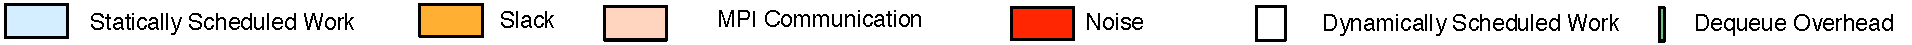
\includegraphics[scale=0.15]{./images/legend-dynamic}\\
 \vspace*{-0.2in}
  \begin{center}
    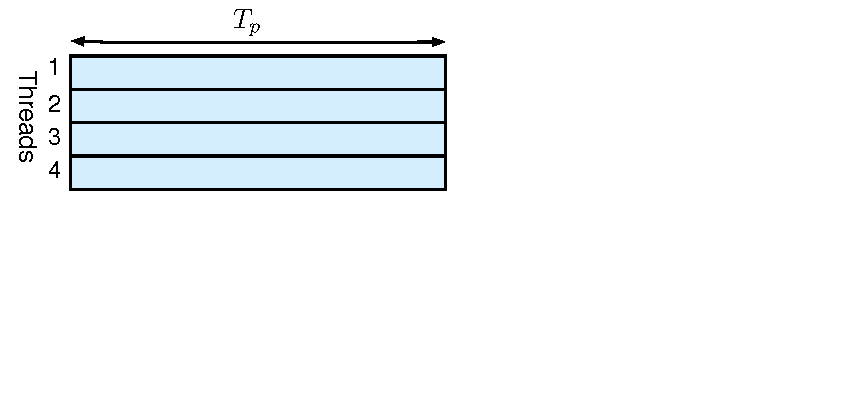
\includegraphics[scale=0.31]{images/threadedCompRegion-static}
  \end{center} 
  \vspace*{-0.4in}
  \begin{center} 
    \tiny Susceptible to imbalance.  
  \end{center} 
\end{columns}
\begin{columns}
\column{0.5\columnwidth}
\vspace*{-0.15in}
\begin{figure}
\lstinputlisting{listings/threadedCompRegion-dynamic.c}
\end{figure}
\column{0.5\columnwidth}
  \begin{center}
    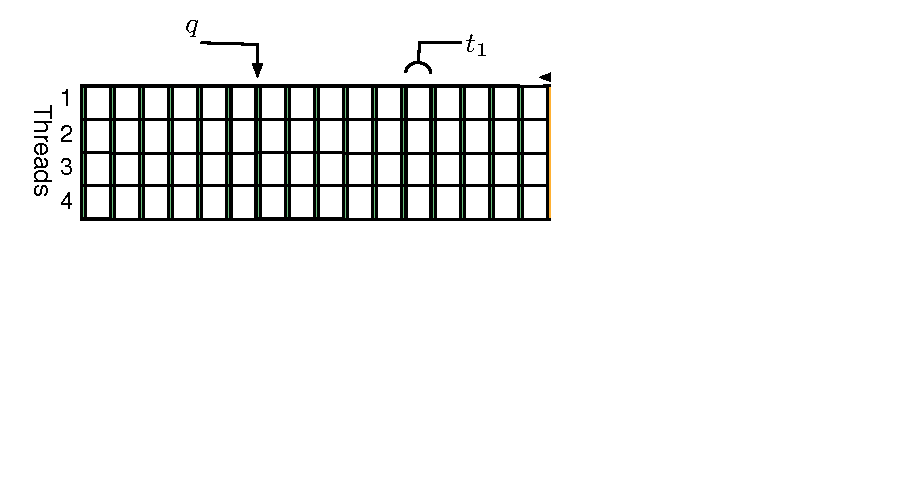
\includegraphics[scale=0.31]{images/threadedCompRegion-dynamic}
  \end{center}
\vspace*{-0.3in}
\begin{center}
{\tiny Scheduler overhead stretches time.}
\end{center}
\end{columns}
\begin{columns}
\column{0.5\columnwidth}
%TODO: fix code  to be hybrid sched
\vspace*{-0.1in}
\begin{figure} 
\lstinputlisting{./listings/threadedCompRegion-hybrid.c}
\end{figure}
\column{0.5\columnwidth}
\begin{center}
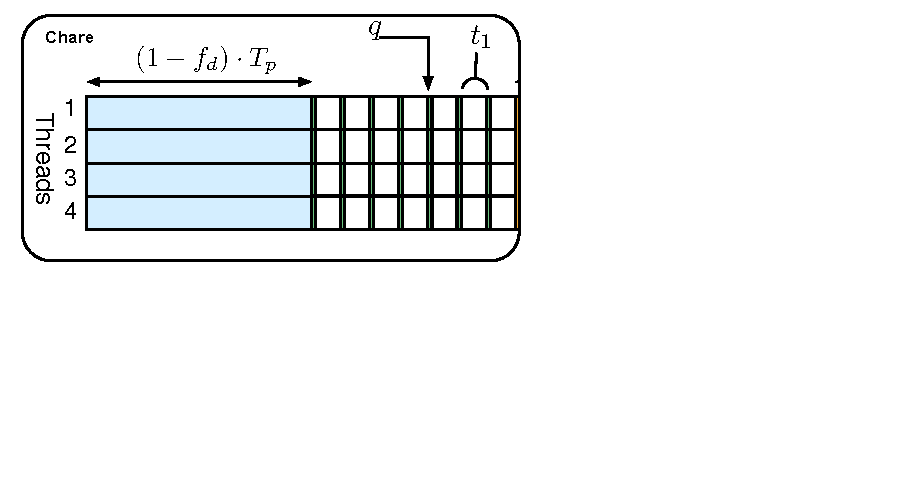
\includegraphics[scale=0.31]{./images/threadedCompRegion-hybrid}
\end{center}
\vspace*{-0.3in}
\begin{center}
{\tiny Can reduce imbalance and sched ovhd. simultaneously.}

%\comments{through \hyperlink{expTunedSF}{tuning} static fraction.}

\end{center}
\end{columns}
\end{frame}

%TODO: experimentally tuned static fraction. 

\begin{frame}[label=besftimings]
\frametitle{Performance with~\hyperlink{expTunedSF}{Tuned} Static Fraction}
\begin{figure}[ht!]
\begin{center}
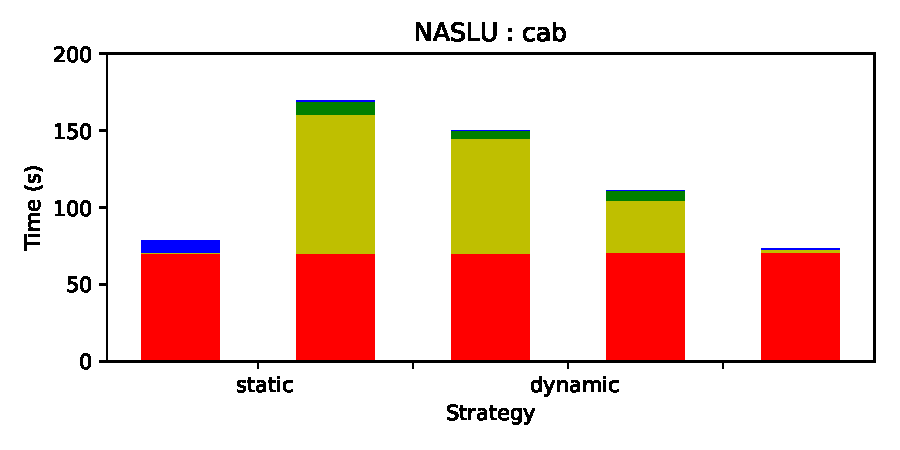
\includegraphics[scale=0.34]{./plots/dmTime-NASLU-cab-withsdandbesf}
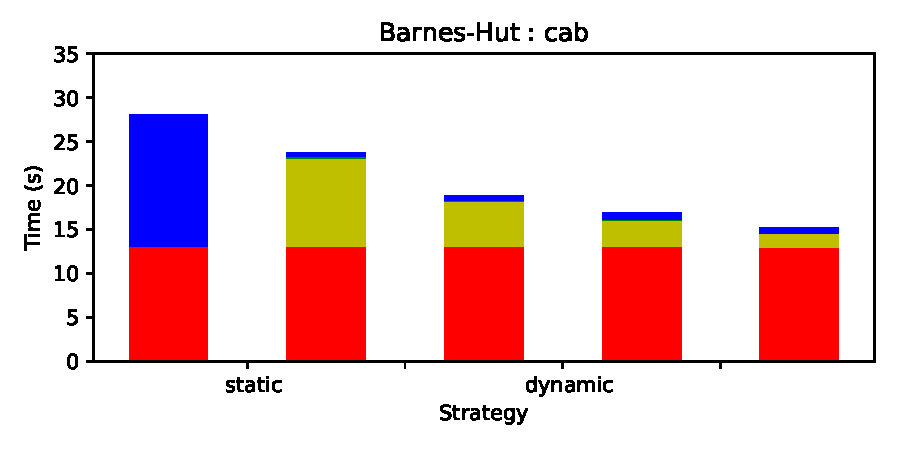
\includegraphics[scale=0.34]{./plots/dmTime-nbody-cab-withsdandbesf}\\
\end{center}
\label{fig:dmTimes-NASLU-cab}
\end{figure}
\begin{center}
{\small In \textit{besf}, we use the best static fraction. See rightmost bar.}
\end{center}
%TODO: fix this so it doesn't duplicate
\visible<1->{
\begin{itemize}
\small \item \small Balances the tradeoff between load balance and locality
 across applications and platforms. \comments{Half is better than dynamic strategies.}
\item \small Even for NASLU, the~\textit{besf} gives performance gains
  over~\textit{static}, i.e., it benefits from the small amount of dynamic load balancing. 
%\item \tiny Minimizes the costs in each of the three challenges,
%simultaneously. 
\item \small EuroMPI 2010: V. Kale and W. Gropp [statdyn] studies this idea in more depth.
\end{itemize}}
\end{frame}

\begin{frame}      
\frametitle{Data Movement with Lightweight Scheduling}
\visible<1->{
\begin{figure}[t]
\label{fig:cacheMisses-cab} 
\begin{center}   
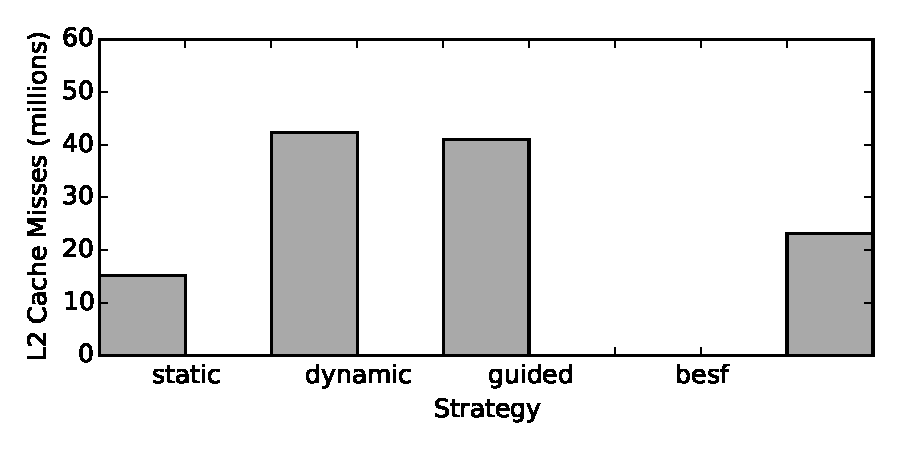
\includegraphics[scale=0.30]{plots/L2-CacheMisses-nbody-cab-withbesf}
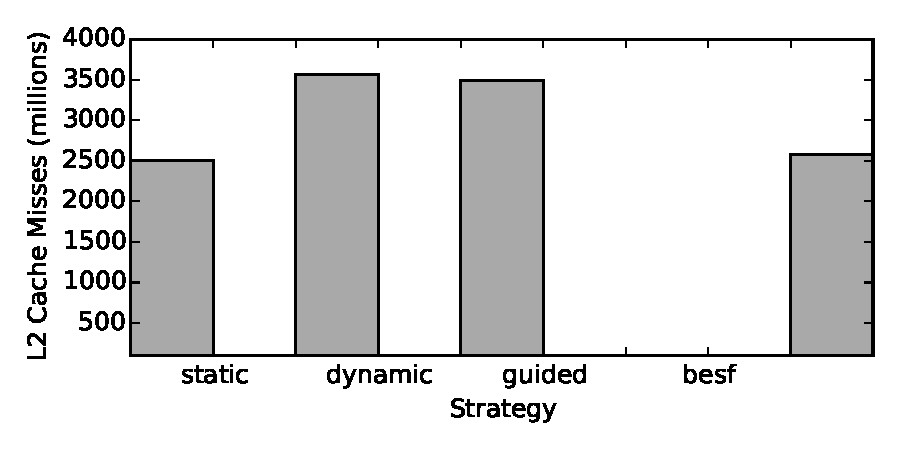
\includegraphics[scale=0.30]{plots/L2-CacheMisses-NASLU-cab-withbesf}\\  
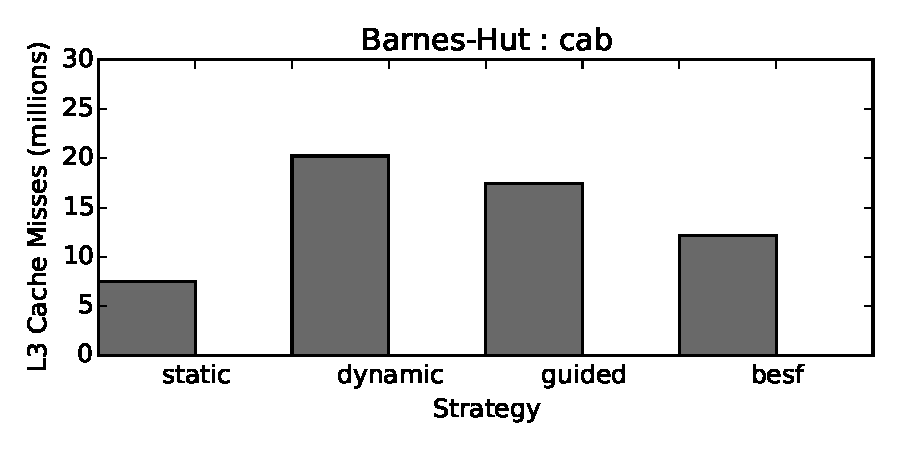
\includegraphics[scale=0.30]{plots/L3-CacheMisses-nbody-cab-withbesf} 
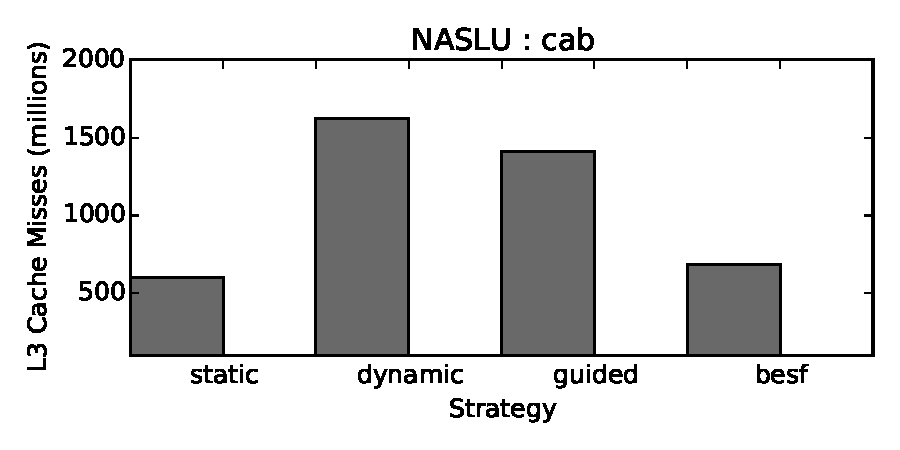
\includegraphics[scale=0.30]{plots/L3-CacheMisses-NASLU-cab-withbesf}
\end{center}
%\caption{\label{fig:cacheMisses-nbody-cab} L2 cache misses (top) and L3 cache misses (bottom).}
\caption{\small Cache misses for \textit{besf}, added on the rightmost bar.}
\end{figure}   
}                             
%\begin{center}     
%The data shown is based on a 100 trials run on a single node of the respective machines. Data movement time is obtained by subtracting the sum of idle time, dequeue time and computation time, from total execution time.  
%}  |
%\end{center}    
\visible<1->{     
\begin{itemize}    
\tiny \item \tiny When using \textit{besf} scheduling, cache misses decrease w.r.t. \textit{half}, for both nbody and NASLU codes. This is   
because we tune to balance the tradeoff between load balance and locality, to minimize the costs in each of the three challenges, simultaneously.  
\item \tiny Paper [statdyn1] studies this idea in more depth.
\end{itemize}}   
\end{frame}                         
%TODO: L3: consider adding already  optimized dense matrix
%factorizations.

\begin{frame}[label=ladmf]{Locality-aware Scheduling for Already Optimized Dense Matrix Factorization}
{\footnotesize Could ensure that threads work on same data from previous invocation of threaded computation region during application execution.}
{\footnotesize Ran CALU with locality-aware Scheduling Schemes on 16-core node using standard compiler flags, thread-to-core pinning.} 
\vspace*{-0.1in}
\begin{figure}
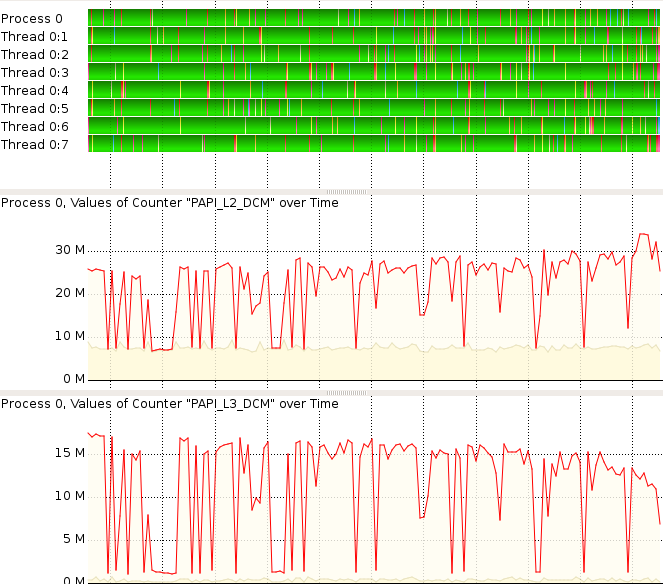
\includegraphics[scale=0.12]{plots/calu_p7_appProfile_dynamicsched.png}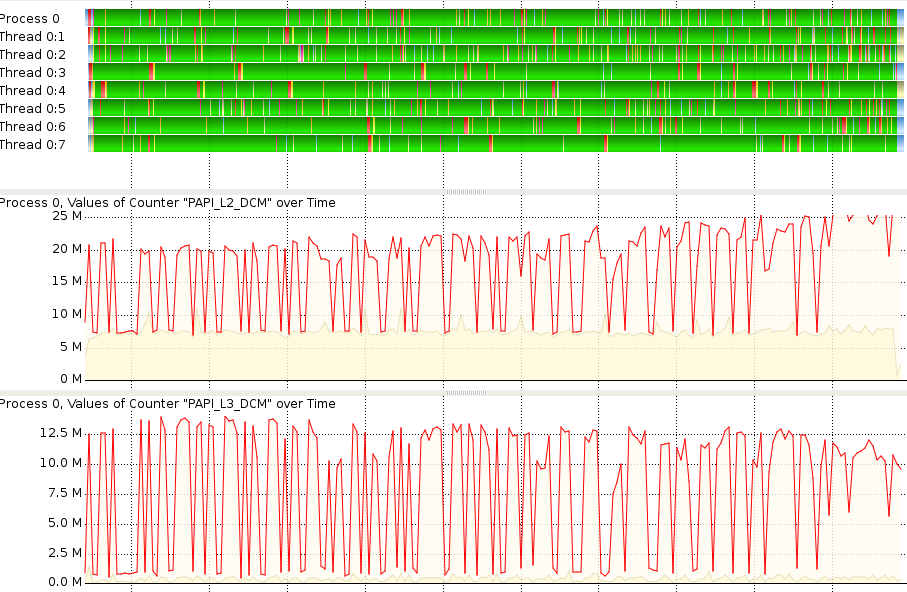
\includegraphics[scale=0.12]{plots/calu_p7_appProfile_locawaresched.png}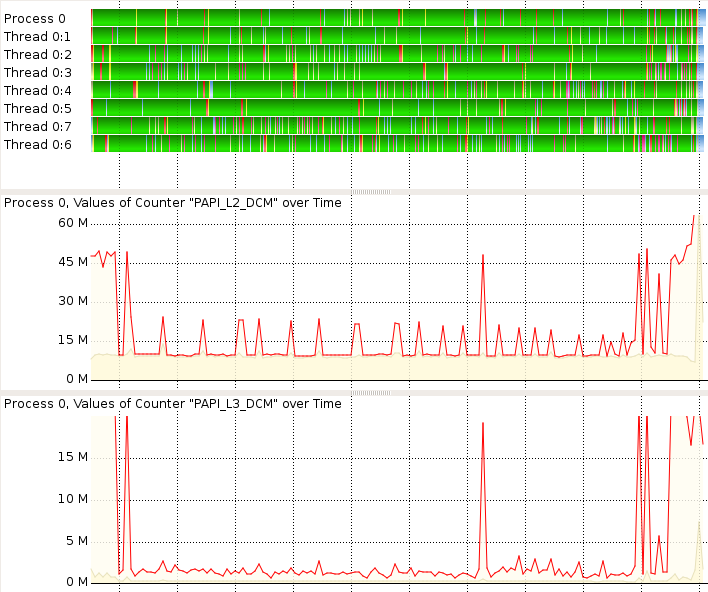
\includegraphics[scale=0.12]{plots/calu_p7_appProfile_locawareopt.png}\\{\tiny Bad data locality, great load balance.}{\tiny Reduced coherence cache misses, moderately good load balance.}{\tiny Even fewer coherence cache misses, good load balance.}\end{figure}\hspace*{0.3in}\begin{figure}[ht!]
\end{figure}
\vspace*{-0.2in}
\begin{itemize} 
\tiny \item \tiny Different solutions provide different balance of load balance and data locality. 
\tiny \item \tiny A solution that works for one application architecture pair may work poorly for another pair.
\item \tiny To get most performance gain, need to tune scheduler for load balance and locality for each application-architecture pair.
\end{itemize} 
\end{frame}

\begin{frame}[label=hybstatdyndmf]
\frametitle{Already Optimized Dense Matrix Factorization Using Hybrid Static/Dynamic Scheduling}
%\framesubtitle{For Problem 1: Does our scheduling approach perform
%competitively or better than other industry wide schedulers?}
\vspace*{-0.2in}
\begin{columns}
\column{0.5\textwidth}
\begin{figure}[ht!] 
%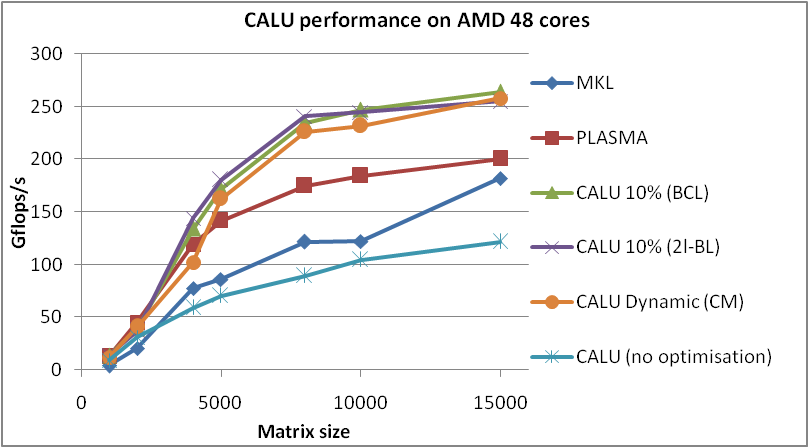
\includegraphics[scale=0.22]{./plots/calu-fastNUMA4-perf}
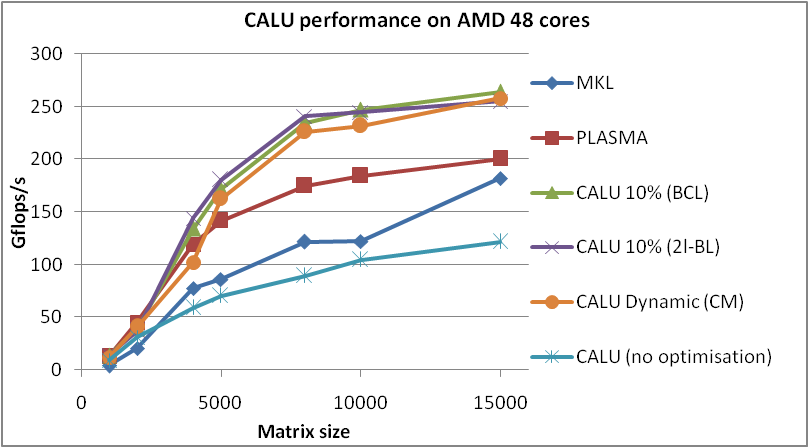
\includegraphics[scale=0.22]{./plots/calu-fastNUMA4-perf}
\caption{\tiny Comparison of hybrid static/dynamic scheduled CALU to original CALU (first version), PLASMA and MKL.\comments{showing significant performance improvements over the baseline (statically scheduled) CALU, particularly with large matrix sizes.}}
%\end{itemize}
%(Problem: PLASMA has inefficient work-stealing algorithm.)
\end{figure}
\column{0.5\textwidth}
\begin{figure}
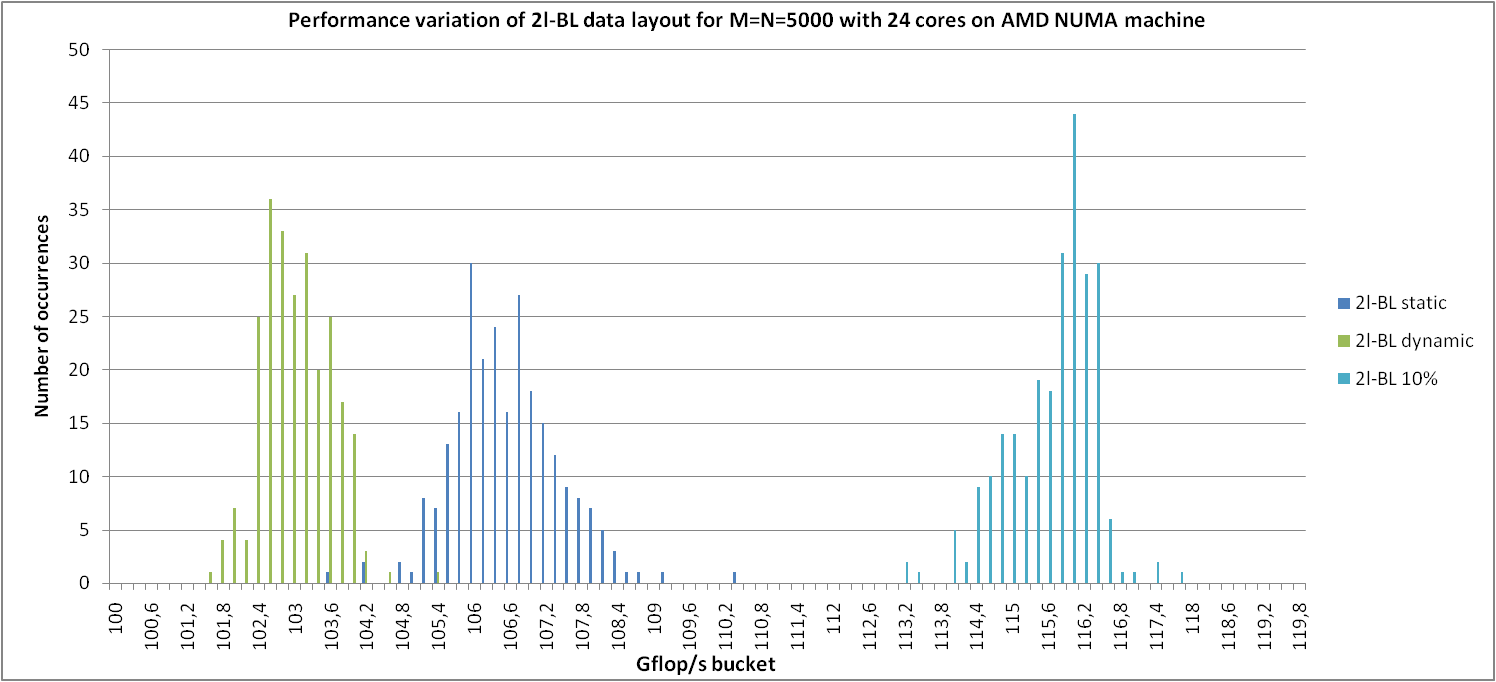
\includegraphics[scale=0.10]{./plots/calu-fastNUMA3-histogram}
\caption{\tiny Performance Variation across runs for static CALU, dynamic CALU, and hybrid static/dynamic CALU.}
\end{figure}
\end{columns}
\visible<1->{
\begin{enumerate}
\small \item \small \comments{$\rightarrow$} 30\% better than PLASMA library's implementation of the same numerical algorithm, and 38\% better than Intel MKL's.
\item \small $\rightarrow$ Performance variability consistent with the performance variability results for 3D stencil.
\end{enumerate}
}
% Significant performance improvements
% over the baseline (statically scheduled) CALU, particularly with large matrix sizes.}
\end{frame}

%TODO: make persistent load imbalance graph
%TODO: see if the below is ok, in terms of older data.       

\begin{frame}
\frametitle{Reduction of Performance Variation Using Lightweight Scheduling}  
\begin{figure}     
%\includegraphics[scale=0.35]{../images/IterTimesHisto-outliers-hybsched.pdf}  
%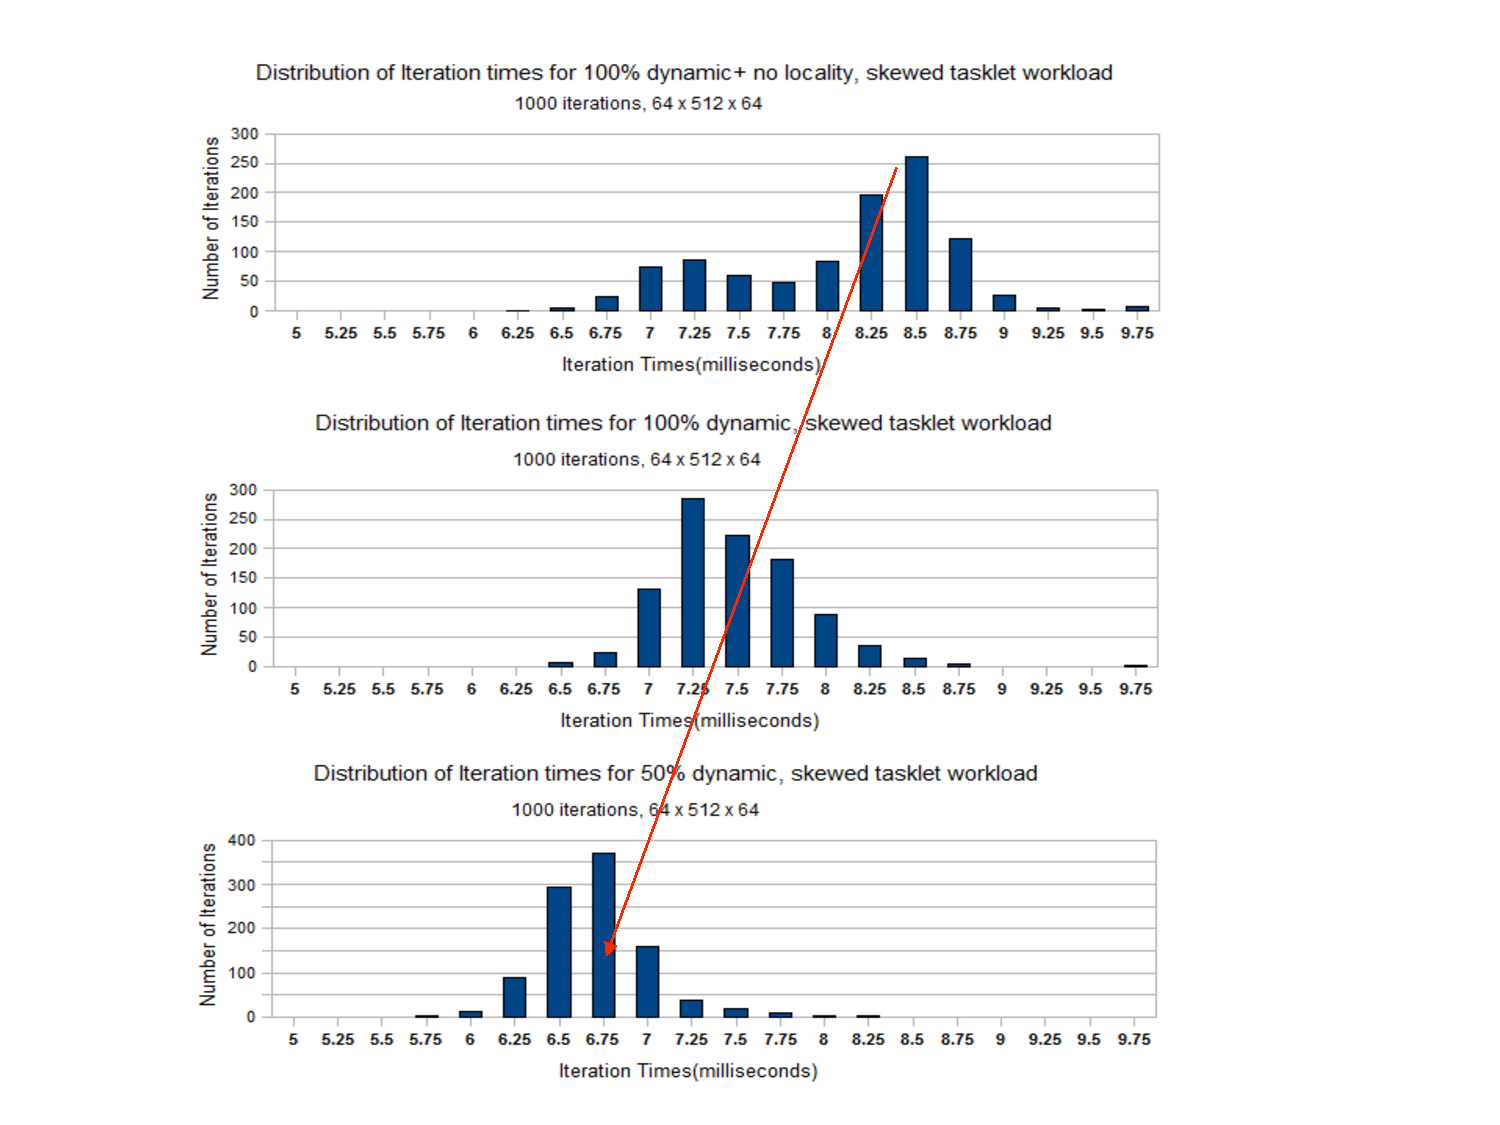
\includegraphics[scale=0.35]{../images/IterTimesHisto-skewedWorkload1.pdf} 
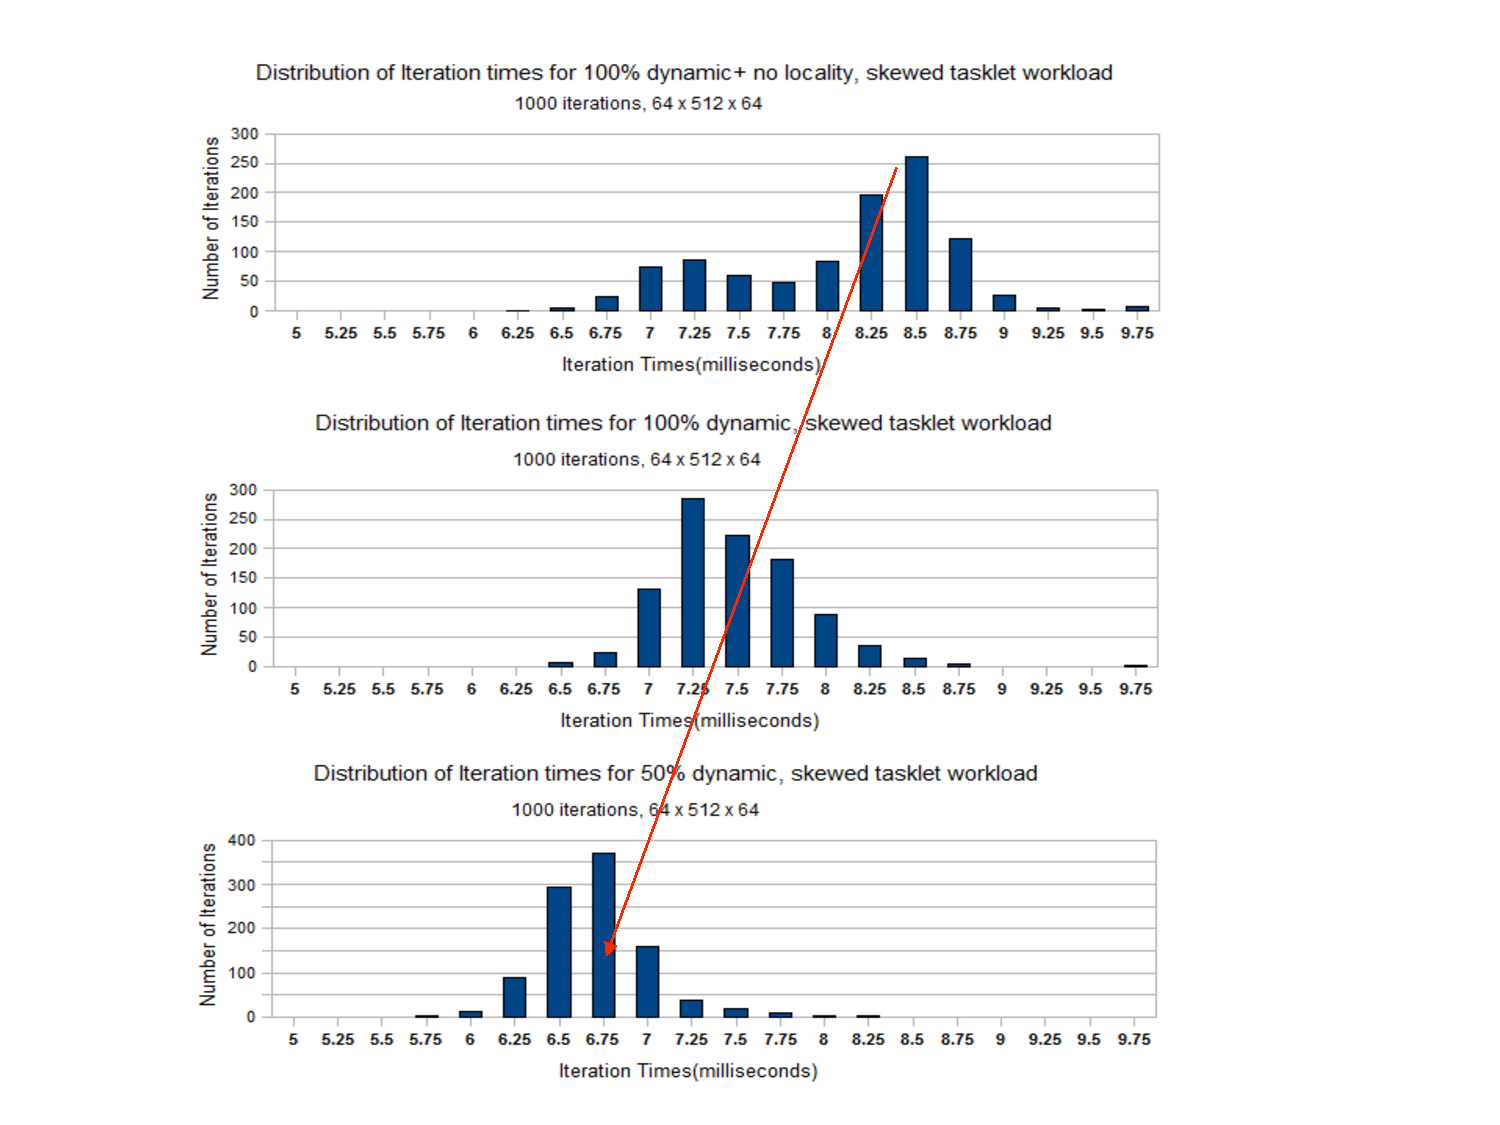
\includegraphics[scale=0.35]{./plots/IterTimesHisto-sdImprovement.pdf} 
%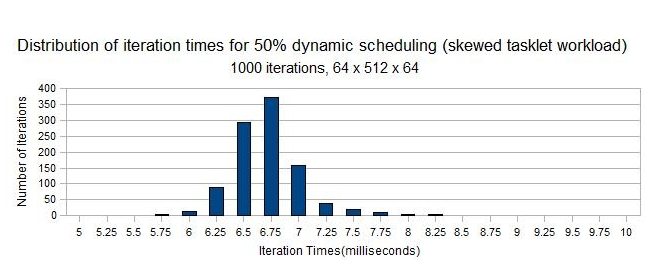
\includegraphics[scale=0.21]{../images/IterTimingsHisto-uSched}   
%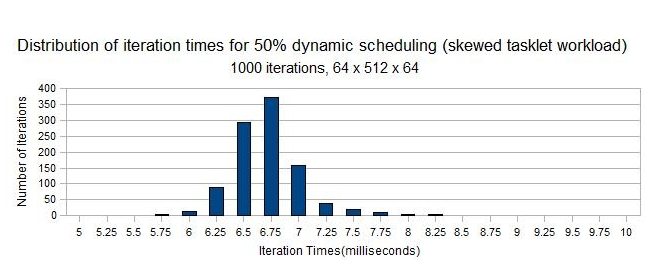
\includegraphics[scale=0.21]{../images/IterTimingsHisto-hybrid}
%\includegraphics[scale=0.15]{../images/stencil-scaling}      
\caption{\small Iteration Timing Histogram for a 3D stencil shown for static scheduling(top) and mixed static/dynamic scheduling (bottom), along with tuned mixed static/dynamic scheduling. Performance variation of 3D stencil is reduced with basic mixed static/dynamic scheduling, seen through the reduction of outliers in the bottom graph.}      
\end{figure}
\end{frame}


\begin{frame}
\frametitle{Improvement of Scalability for 3D stencil} 
%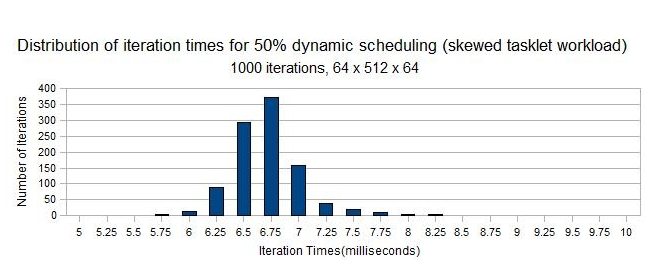
\includegraphics[scale=0.21]{../images/IterTimingsHisto-uSched}
%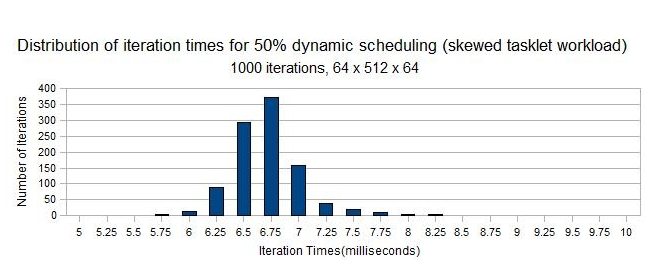
\includegraphics[scale=0.21]{../images/IterTimingsHisto-hybrid}
\begin{figure}
\vspace*{-0.15in}
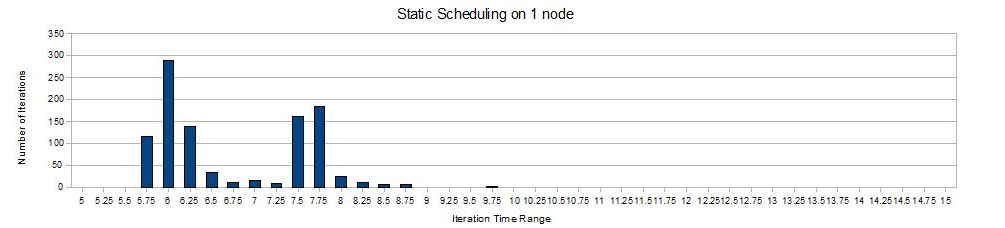
\includegraphics[scale=0.17]{plots/scaling-histograms-stat1.png} 
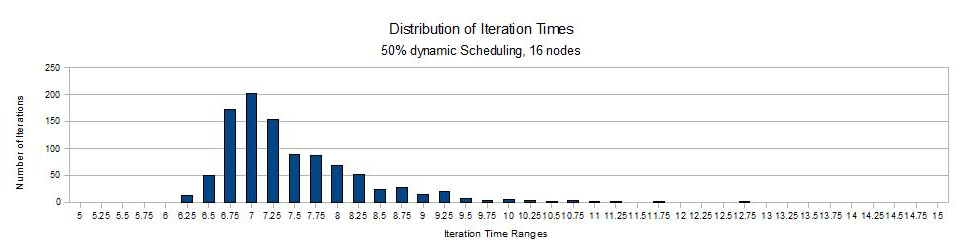
\includegraphics[scale=0.17]{plots/scaling-histograms-statdyn16.png}
\caption{\small Iteration Timing Histogram for 3D stencil shown for static scheduling (left) and mixed static/dynamic scheduling(right) at 64 nodes of IBM Power5+. The reduction of performance variation using mixed static/dynamic scheduling    
results in improved scalability.}
\end{figure}  
\end{frame}     

%TODO: Discuss the relevant reference(s)/paper(s)
\begin{frame}[label=problemBasicHybStat]
\frametitle{Challenges and Extensions to Hybrid Scheduling}
%\textbf{Two problems with the above basic approach:}
\begin{enumerate}
%\small \item \small Load imbalances across cores could be a mixture
%of transient and persistent.
  %How do we handle both persistent and transient imbalances together? 
\item Search space for tuning the scheduler is large and complex.
  \begin{itemize} 
  \item Develop analytical model to predict optimal static fraction. [NLAopt12]
  \end{itemize}
\item \textbf{Slack} in collective operations: presents an opportunity. 
\item \textbf{Spatial locality} in dynamic iterations disturbed, and not as good as static scheduling.
%Our scheduling methodology improves temporal locality, but it
%actually disturbs spatial locality disturbed. 
%Our scheduler does not consider spatial locality
\end{enumerate}
\end{frame}

%TODO: figure out whether we need to use coupling. 
%TODO: word the below better                                                           
\begin{frame}
\frametitle{Problem 1: Persistent Load Imbalances Not Handled}
\begin{figure}
%\includegraphics[scale=0.44]{../images/noise_pes_jaguar}         
\subfloat[\small Jaguar quasi-persistence in noise.]{\includegraphics[scale=0.41]{./plots/noise_pes_jaguar}}
\subfloat[\small Ranger quasi-persistence in noise.]{ 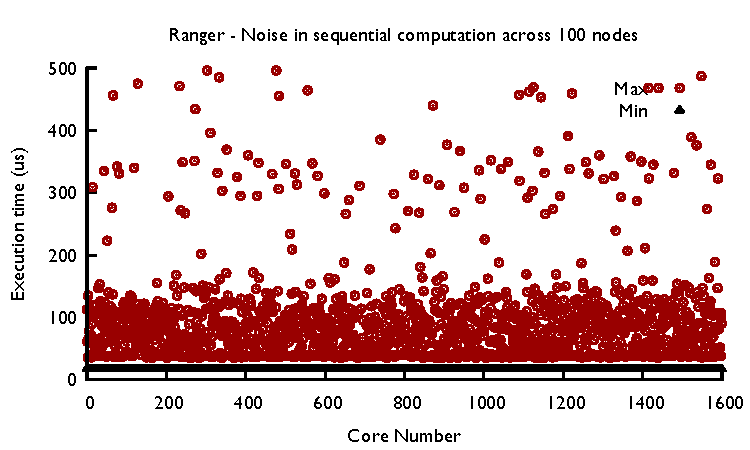
\includegraphics[scale=0.41]{./plots/noise_pes_ranger}}
\caption{\small Load imbalance (here shown due to noise) can be persistent, not just transient.}
\end{figure}
\end{frame}
%TODO: check the question presented in the title of the slide 

%TODO: get another graph - this may not show the results as well.                  
%TODO: show a caption.       
\begin{frame}
\frametitle{Problem 2: Search Space is Too Large}
%TODO: get new picture. 
%Also, Could maybe show results for enumeration of search space, and that it's large here.         
%TODO: fix the below.          
\begin{figure}
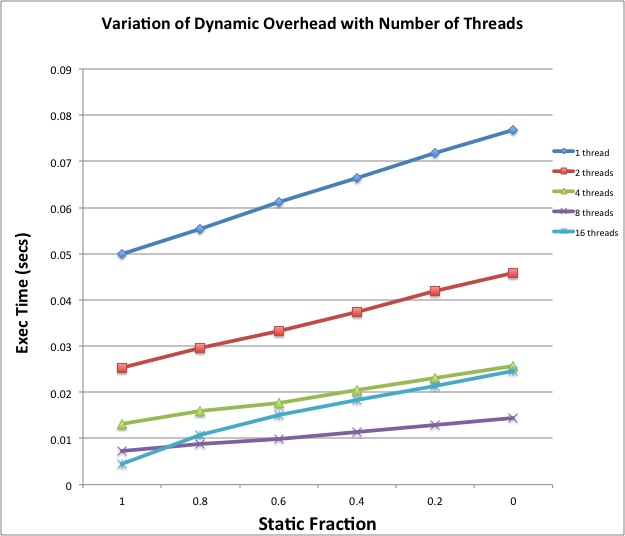
\includegraphics[scale=0.20]{./plots/vary-sf-for-diff-threads}
\caption{Graph showing the performance of different static fractions used. Here, we have tried different static
fractions, in increments of 0.1. The minima here is difficult to attain.}
%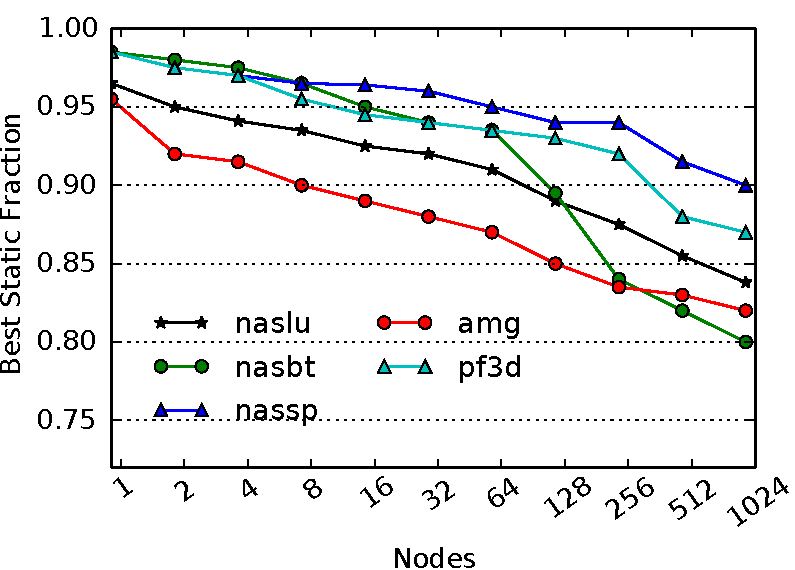
\includegraphics[scale=0.28]{../plots/best-fs-vs-nodes}
\end{figure}
\end{frame}

\begin{frame}
\frametitle{Different Slack Across Different Processes}
\vspace*{-0.3in}

\begin{table}[tr]
\label{fig:collectiveSlack-useq}
  \begin{center}
    \begin{tabular}{ | c || c | c || c |  }
      \hline
      \textbf{Collective}  &      \textbf{max} & \textbf{avg ($\sigma$)} & \textbf{$\sigma_i$}  \\ \hline
      \texttt{Allreduce} &             307    &    199 (.792) &            .102                  \\ \hline
      \texttt{Alltoall}  &             280    &    149 (.821) &            .176                  \\ \hline
      \texttt{Barrier}  &              250    &    139 (.178)  &           .061                  \\ \hline
      \texttt{Allgather} &             268    &    189 (.527) &            .115                  \\ \hline
      \texttt{Reduce\_scatter} &       459    &    296  (.649)  &          .129                  \\ \hline
    \end{tabular}
  \end{center}
  \caption{\label{fig:collectiveSlack-useq}
    Slack statistics (in $\mu$s) across MPI processes.}
{\small Slack consistent across iterations, and diff. across MPI processes } \\
%(2nd and 3rd column) and standard deviation across processes iterations (4th column) of a 512 process execution of specific collective operations %on uSeq.
\end{table}
{\small $\rightarrow$ makes cost of lightweight scheduler on critical path different for different MPI processes.} 
\end{frame}

\begin{frame}
\frametitle{Problem: Only Handle One Dimension of the Tradeoff between Locality and Load Balance.}

\begin{figure}[ht!]
\begin{center}
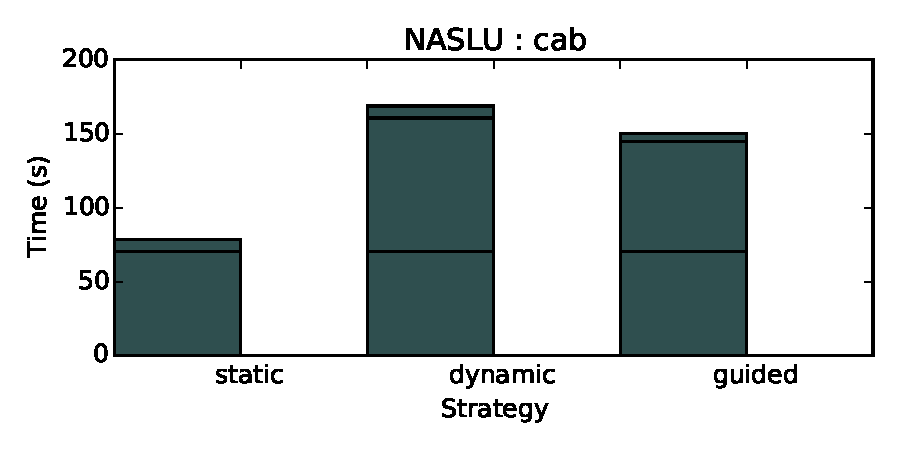
\includegraphics[scale=0.26]{plots/baseline-NASLU-cab-wallTime.pdf}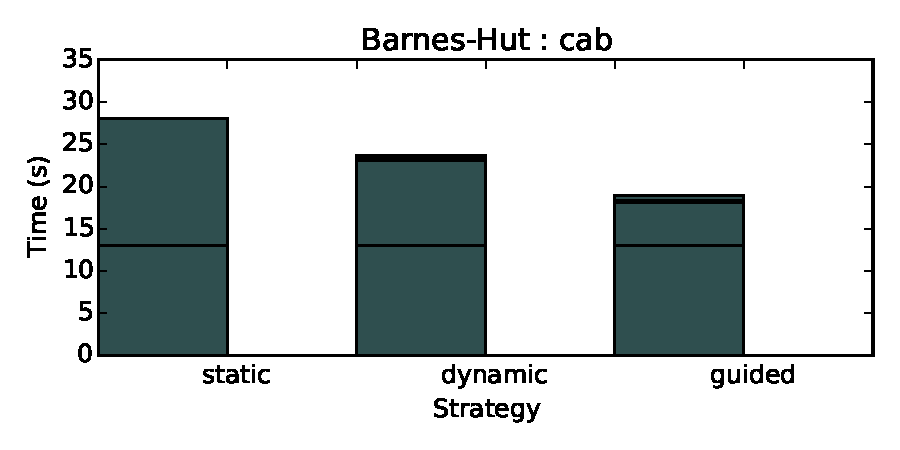
\includegraphics[scale=0.26]{plots/baseline-nbody-cab-wallTime.pdf}
\end{center}
\end{figure}

\begin{center}
{\small Shows evidence that spatial locality is lost when using our standard mixed static/dynamic scheduling strategy for {\tt rzuseq} (left) and \texttt{cab} (right).}
\end{center}
\end{frame}

\begin{frame}[label=weightedlss]{Weighted Locality-sensitive Scheduling}
\begin{columns}
\begin{column}{0.5\columnwidth}
\centering
%\begin{column}{0.5\columnwidth}
%\fbox{
\begin{figure}[ht!]
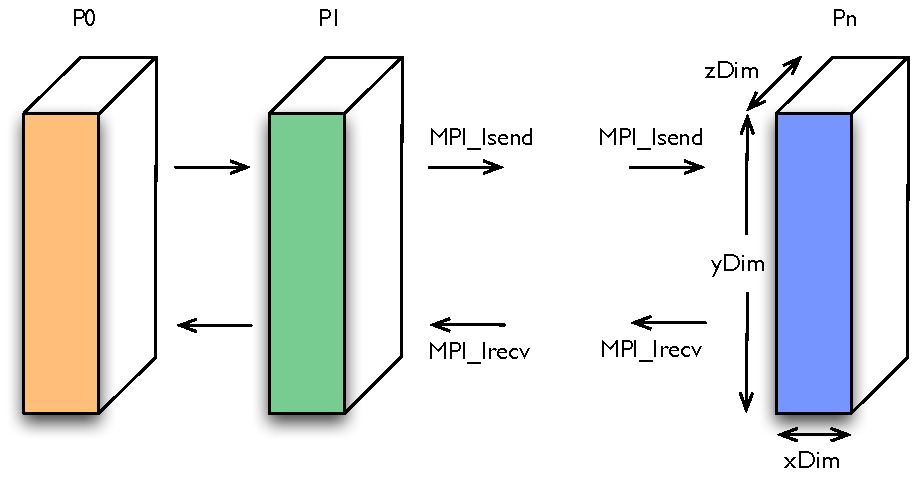
\includegraphics[width=0.5\columnwidth]{images/mpi_decomp-diff-proc-color}
\end{figure}
%}
%\end{column}
%\begin{column}{0.5\columnwidth}
\visible<1>{
%\fbox{
\begin{figure}[ht!]
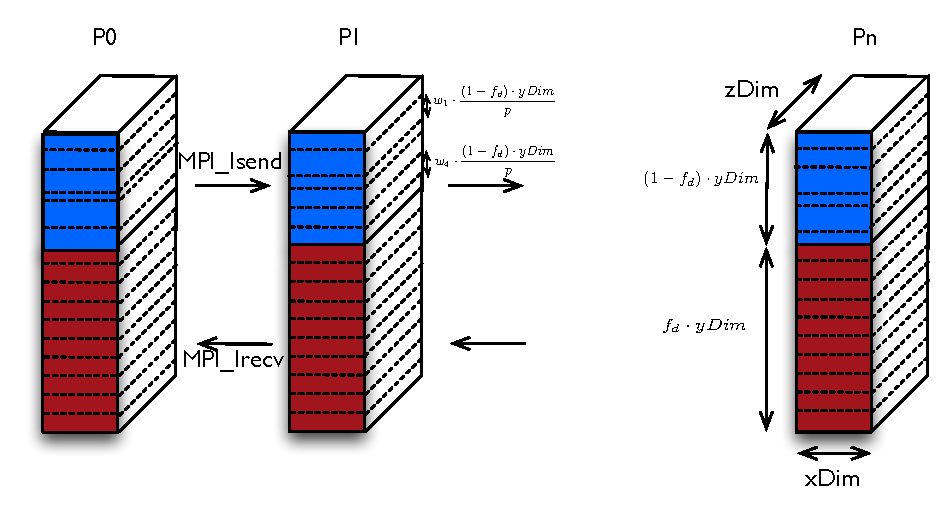
\includegraphics[width=0.5\columnwidth]{images/weighted_decomp}
\end{figure}
%}
}
\end{column} 
\end{columns}
\end{frame}

\begin{frame}[label=slackfs]
\frametitle{Slack-Conscious Hybrid Static/Dynamic Scheduling}
%\comments{(a.k.a. Adaptive Scheduling)}} 
% {\small Extend analytical model and use callsite history to predict lack.}
\begin{center}
{\small $\delta$ is the length of perturbance.} 
\end{center}
% TODO: describe the variables. 
\begin{figure}
  \begin{center}
    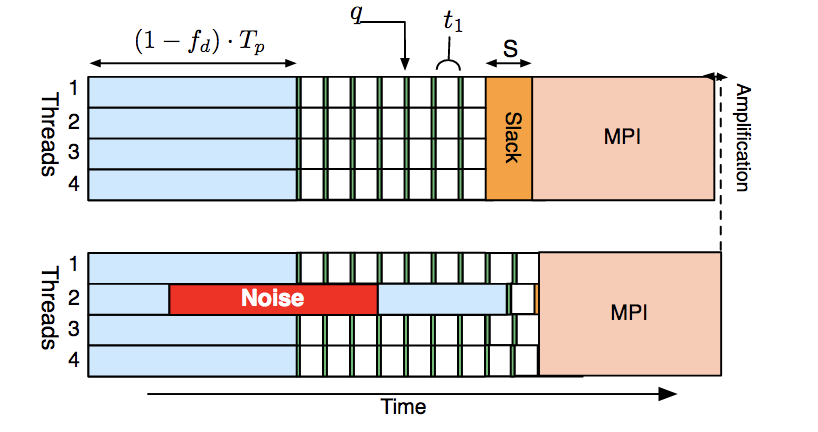
\includegraphics[scale=0.41]{./images/slackConsciousSched}
  \end{center}
\end{figure}
\begin{center}
\fbox{{$f_d = \frac{p\delta}{N\left(t_1 + q\right)}$}}
\fbox{{$f_d' = f_d - \frac{S}{(p-1)\frac{Nt_1}{p} - Nq}$}}
\end{center}
\begin{center}
{\tiny Note that $f_d'$ and $S$ are local variables within each MPI process.}
\end{center}

%TODO:
%\small \item \small Given slack, can we reduce the dynamic fraction

\begin{itemize}
\small \item \small Slack allows us to reduce the dynamic fraction
further. \comments{, because a small amount of delay due to noise will lead to no delay in the completion of an MPI collective operation.}
\begin{itemize}
\tiny \item \tiny The dynamic fraction $f_d$ of a particular node is reduced by a value proportionate to the slack on that node, to get the new $f_d'$.
\end{itemize}
\end{itemize}
\end{frame}

%\begin{frame}[label=sa]{Software Architecture}
%\begin{figure}[ht!]
%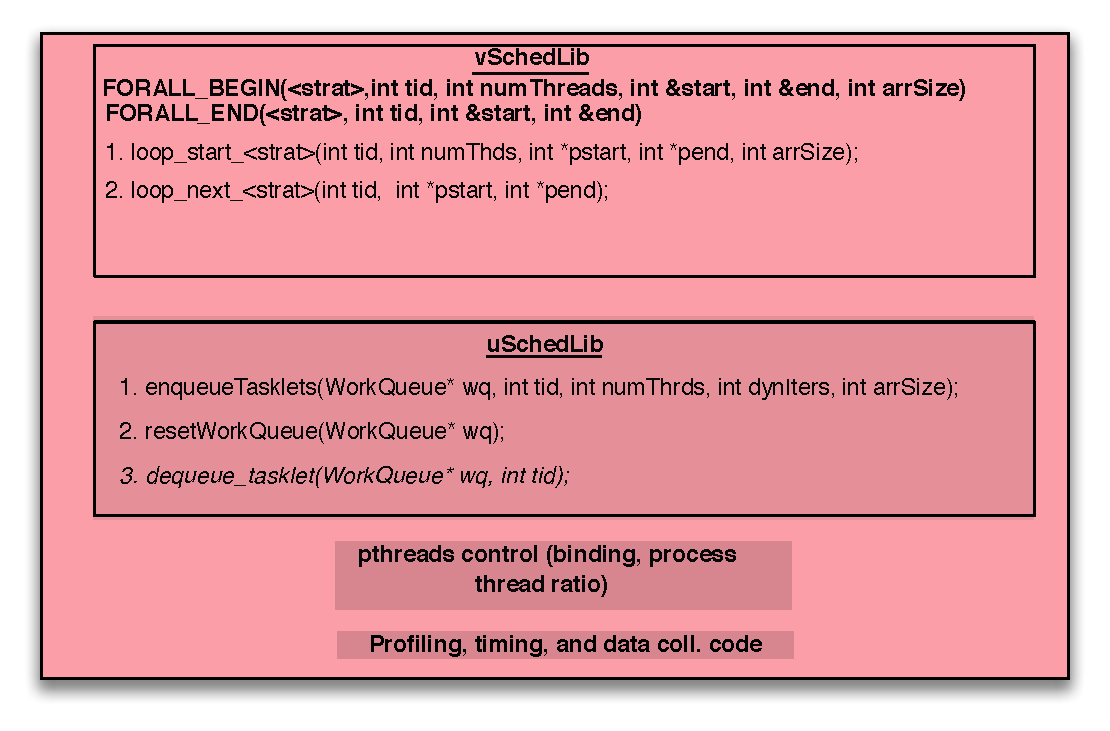
\includegraphics{images/architecture}
%\caption{Software Architecture for loop scheduling techniques.}
%\end{figure}
%\end{frame}

%\begin{center}
%{\small How to implement slack prediction and adjustment?}\\ 
%\end{center}
%{\small To estimate the slack on each processor, we use ideas from
% Adagio (see next slide for impl).\\ We compared multiple methods.
% and chose the \textit{callsite\_fd} method.} \\
%{\small Reducing dynamic fraction reduces overall overhead.} 

\begin{frame}[label=softwareArch]
\frametitle{Software Architecture}
\begin{figure}[ht!]
\begin{center}
\label{code:architecture}
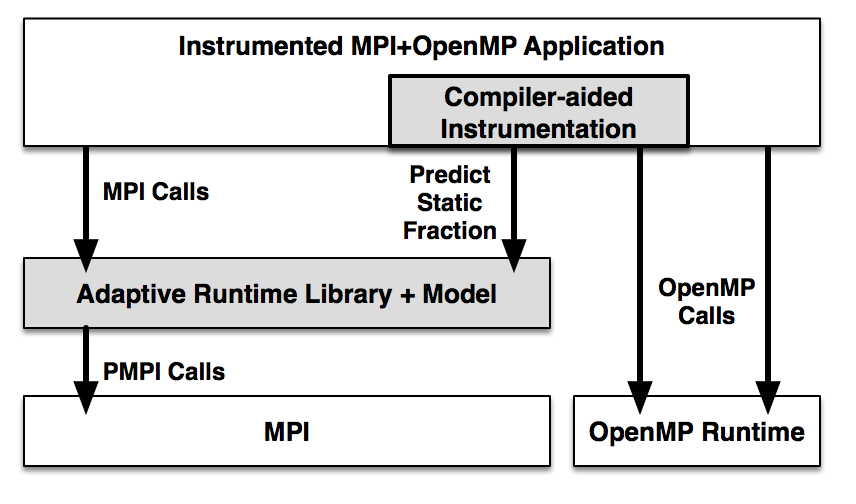
\includegraphics[scale=0.56]{images/architecture.png}
\end{center}
\end{figure}
\begin{itemize}
\tiny \item \tiny The white rectangles taken by themselves show the interaction between the MPI+OpenMP application code and the
MPI \& OpenMP runtimes.
%how a basic MPI+OpenMP application is run. 
\item \tiny Our contributions in this work are shown in gray rectangles. %Involves source-to-source transformation and adaptive
\item \tiny Predict static fraction call (arrow going from Compilation to Adaptive Runtime Library) is how MPI runtime communicates with OpenMP runtime to tune OpenMP scheduler parameters (and other parameters).
\end{itemize}
\end{frame} 


%TODO:L2/L3: figure out where this should be introduced. 
\begin{frame}[label=sdsSched]
\frametitle{Improving Spatial Locality by Staggering}
\begin{center}
\includegraphics[scale=0.28]{./images/sdIncrIters}
\end{center}
\begin{itemize}
\small \item \small Each thread finishes its static iterations.
\item \small Then does dynamic iterations marked for it if available.
\item \small Only if not, looks for other dynamic work from other threads to steal.
\end{itemize}
%\column{0.55\columnwidth} 
\begin{center}
%\begin{figure}
\includegraphics[scale=0.28]{./images/sdsIncrIters}
%TODO: update the below, to word better for intent.                         
%\caption{\tiny We stagger the dynamic iterations in order to improve 
%  spatial locality of the hybrid static/dynamic scheduling.} 
%\end{figure}
\end{center}
\begin{itemize}
\item \small Spatial locality won't be lost in common cases:
\begin{enumerate}
\tiny \item \tiny no imbalance
\item \tiny Even for single-core imbalances, e.g., noise: most
 threads are able to complete their own dynamic iterations.
%\item \tiny Even when there is imbalance
\end{enumerate}
\end{itemize}
%\end{columns}
\end{frame}

\begin{frame}[label=schedComp]
\frametitle{Scheduler Composition}
\begin{itemize}
%\tiny \item \tiny Some schedulers may benefit in some cases, others
%elsewhere.
%\small \item \small Each scheduler handles a subset of factors.                  
\small \item \small Problem: Machine and application have many
different mentioned factors involved, esp. as we go to exascale.
\item \small We see if we can compose schedulers to handle all factors and circumstances.
\end{itemize}
\end{frame}

\begin{frame}[label=combinedSched]
\frametitle{Components of Example Composed Scheduler}
%\begin{columns}
%\column{0.5\columnwidth}
\begin{itemize}
\small \item \small \textbf{hybSched}: hybrid static/dynamic scheduling
with static fraction exposed to user.\\
%TODO : below is level 2 composition 
\item \small \textbf{uSched}: Use model-guided optimization to
  determine the static fraction,  and then experimentally tune the
  static fraction $0.05$ below static fraction and $0.05$ above static
  fraction ($0.05$ is a configurable parameter).
\item \small \textbf{slackSched}: Starting with \textit{uSched},
adjusting the static fraction on each process based on its slack.
\item \small \textbf{vSched}: Use static fraction from \textbf{uSched},
  and then stagger iterations for spatial locality in dynamic
  iterations.
\item \small \textbf{comboSched}: Start with the staggered static/dynamic scheduling scheme defined in \textbf{vSched} above, and then do the slack-conscious adjustment described in slack-conscious scheduling section.
\end{itemize}
\end{frame}

\begin{frame}[label=appsAndExpSetup]
\frametitle{Application Codes Description\comments{and Experimental Setup}}
\begin{itemize}
\small \item \small {\bf SNAP:} Regular mesh computation, 
implementation done in MPI+OpenMP, used for heat diffusion simulation.
\item \small {\bf miniFE:} Finite element unstructured mesh computation, implementation done in MPI+OpenMP, used for earthquake simulation. 
\item \small {\bf Rebound:} N-body computation, implementation
  MPI+OpenMP, used for bio-molecular interaction simulation.
%(our
% specific example input and code instance simulates particle-particle
% interactions in Jupiter's ring). 
\end{itemize} 
\end{frame} 

\begin{frame}[label=combinedregmesh]
\frametitle{Scheduling Strategy\comments{Composition} Results for \textit{SNAP}}
{\tiny CORAL MPI+OpenMP \textit{SNAP} heat diffusion code performing regular mesh sweep.}
\begin{figure}[ht!]
\includegraphics[scale=0.38]{./plots/app-scaling-strat-SNAP-fastNUMA2}
\caption{\tiny Percent speedup over OpenMP static scheduling for
  different loop scheduling strategies.}
\end{figure}
\begin{itemize}
  \small \item \small Even when dynamic strategies worsen performance, the combined strategies show a small benefit.
\item \small Optimizations in composition don't cancel each other out; combo sched gets 7.2\% gains over \textit{uSched}.
\end{itemize}
\end{frame}

\begin{frame}[label=combinednbody]
\frametitle{Scheduling Strategy\comments{Composition} Results for\textit{Rebound}}
{\tiny MPI+OpenMP molecular dynamics code performing n-body force
computation. Involves large load imbalances as well as irregular data
access patterns.}
\begin{figure}
\includegraphics[scale=0.38]{./plots/app-scaling-strat-nbody-fastNUMA2}
\caption{\tiny \textit{Rebound} Percent speedup over OpenMP static
  scheduling for
  different scheduling strategies. Code change: 41,421 loc to 41,982
  loc (5.2\%).}
\end{figure}
\begin{itemize}
\tiny \item \tiny Different techniques of \textit{vSched} and
\textit{slackSched} in the \textit{comboSched} don't cancel benefit
out, and composition seems to be additive.
\item \tiny Better combination could lead to even more improvement.
\end{itemize}
\end{frame}

\begin{frame}[label=combinedfe]
\frametitle{Scheduling Strategy\comments{Composition} Results for \textit{miniFE}}

{\tiny CORAL miniFE MPI+OpenMP code of unstructured mesh performing a finite element method. On each timestep, the number of mesh points updated for each compute element is different due to abnormal geometry.}
\begin{figure}[ht!]
\includegraphics[scale=0.38]{./plots/app-scaling-strat-fe-fastNUMA2}
\caption{\tiny Pct. speedup over OpenMP static scheduling for each
scheduling strategy applied to miniFE. Code change: 102,341 loc to 102,667 loc (less than 1\%).}
\end{figure}
\vspace*{-0.2in}
\end{frame}

\begin{frame}[label=perfComp]
\frametitle{Performance with Scheduler Composition} 
\vspace*{-0.13in}
\begin{columns}
\column{0.35\columnwidth}
\begin{itemize}
\small \item \small Optimizations always improve over \textit{uSched}. 
\item \small Combining different techniques seems to add on benefits, i.e., they don't cancel benefit out. 
%\item \tiny Because they are based on complementary factors. Spatial
%  locality in the static/dynamic scheduling vs. reducing dynamic
%  scheduling. 
\item \small Do better than guided. 
\item \small Small code change, e.g., 41,421 loc to 41,982 loc (5.2\%) for Rebound. 
%\item \tiny better combination could lead to even more improvement 
\end{itemize}
\column{0.65\columnwidth} 
\begin{figure}[ht] 
\begin{center} 
\includegraphics[scale=0.18]{./plots/app-scaling-strat-SNAP-fastNUMA2}\\
\vspace*{-0.16in}
{\tiny SNAP reg. mesh code.}
\end{center}

\begin{center}
\includegraphics[scale=0.18]{./plots/app-scaling-strat-fe-fastNUMA2}\\
\vspace*{-0.16in}
{\tiny miniFE unstructured mesh code.}
\end{center}

\begin{center} 
\includegraphics[scale=0.18]{./plots/app-scaling-strat-nbody-fastNUMA2}\\
\vspace*{-0.16in}
{\tiny Rebound N-body code.}
\end{center}
\end{figure} 
\end{columns} 
\end{frame}

\begin{frame}[label=relatedWork]
\frametitle{Related Work}
\begin{itemize}
\small \item \small OpenMP loop scheduling: Chapman, Sarkar, deSupinski.
%PIPES from Sarkar 
% Understanding perf interference in next generation systems from sandia.
% Model for - helps to generate solutions  %TODO:L4: consider whether
% this goes in introduction work also?
% Edgar Leon : 
% Perilla 
% Cespa 
\item \small Task Scheduling:  Work-stealing/Cilk: Leiserson and group at MIT, TBB. 
\item \small DPLASMA. 
\item \small Hybrid MPI+OpenMP or MPI+X. 
\item \small Co-scheduling: Schedule all events together to make only some timesteps be impacted by noise, but can't co-schedule all events.
\end{itemize}
%*Some work/discussions have been done to integrate our scheduler into
%this runtime                                                   
\end{frame}  

\begin{frame} 
  \frametitle{Conclusions} 
  \begin{itemize} 
  \item \small Performance Irregularity difficult to handle through conventional techniques due to complex chain of dependences in MPI collectives.
  \item \small Locality-aware mixed static/dynamic scheduling provides a way to cost efficiently handle the load imbalance induced by performance irregularity  
  \item \small Formalization and Numerical Linear Algebra Application Case Studies  
  \item \small Optimizations: adaptive per-thread static fraction, slack-conscious static fraction.
  \item \small Feasible to integrate into applications through compiler and adaptive runtime.
  \item \small If slowdowns due to performance irregularity are small, our runtime does not induce overheads.  
%  \item \small Can further refine accuracy of slack prediction through risk model. 
%  \item \small Plan to provide more loosely coupled interface between OpenMP and MPI, or between any two programming models. 
  \end{itemize}      
\end{frame}

%TODO: figure out if we should add ``questions'' slide.
%\input{thanks}
%People involved in the project 
%\input{people} 
